%\documentclass[jkps,preprint,fleqn,showpacs,showkeys]{revtex4}
%Modified by Chawon Park
\documentclass[jkps,preprint,fleqn,showpacs,showkeys,10pt,twocolumn]{revtex4}

\usepackage[pdftex]{graphicx}
\usepackage{amssymb}
\usepackage{amsmath}
\usepackage{bm}
%------------------------------------------------------------
% Added by Author (Chawon Park)
\usepackage{color,hyperref}
%    \catcode`\_=11\relax
%%    \newcommand\email[1]{\_email #1\q_nil}
%    \def\_email#1@#2\q_nil{%
%      \href{mailto:#1@#2}{{\emailfont #1\emailampersat #2}}
%    }
%    \newcommand\emailfont{\sffamily}
%    \newcommand\emailampersat{{\color{red}\small@}}
%    \catcode`\_=8\relax    
%------------------------------------------------------------

%Added by Author (Chawon Park)
%\renewcommand{\abstractname}{} % clear the title of abstract
\renewcommand{\abstractname}{\vspace{0.0cm}} % clear the title of abstract

\begin{document}
%\setcounter{page}{0}
\setcounter{page}{1}
%\title[]{Beam Tracking Simulation Study by Using a Three Dimensional Field Map for Multipole Magnets at the HEBT in the KHIMA Accelerator System}
%\title[]{Beam Tracking Simulation Study Using Three Dimensional Field Map of Multipole Magnets at the HEBT in the KHIMA Accelerator System}
\title[]{Beam Tracking Study Using Three Dimensional Field Map of Multipole Magnets at a Medical Synchrotron System}
\author{Chawon \surname{Park}}
\email[E-mail: ]{parknkim@kirams.re.kr}
\author{Heejoong \surname{Yim}}
\author{Dong Hyun \surname{An}}
%\email[E-mail: ]{ectroan@kirams.re.kr}
%\thanks{Fax: +82-2-970-1332}
\affiliation{Division of Heavy Ion Accelerator, Korea Institute of Radiological \& Medical Sciences, Seoul
  139-706}
%\date[]{Received 30 December 2016}
%---------------------------------------------------------------------------------------%
\begin{abstract}
  The Korea Heavy Ion Medical Accelerator (KHIMA) project of Korea Institute of Radiological \& Medical Sciences (KIRAMS) has been engaged in
  designing synchrotron-based ion beams treatment facilities for cancer treatment and various nonclinical scientific research.
  Designed machines can accelerate proton beams from 60 MeV to 230 MeV
  and carbon beams from 110 MeV/u to 430 MeV/u in fine energy variation steps, respectively.
  The particle beams extracted from the Synchrotron are transferred into each treatment room via a dedicated high energy beam transport (HEBT) lines.
  The HEBT line's lattice design was implemented with beam optics codes, MAD-X and WinAgile.  
  The beam tracking code TRACK that covers the whole HEBT line lattice is performed to confirm if the beam loss is arisen in each HEBT line.  
  In order to apply the realized multipolar magnet field into the TRACK code, a three-dimensional field map obtained by the Opera3D program was used.
  By applying a realistic field map of multipole magnets to the TRACK code in the particle beam line,  
  the beam width with respect to various beam energy was deformed by comparing the estimated one from optics code.
  In this analysis, corrections were followed to eliminate the discrepancy between the reconstructed beam width by TRACK
  and the estimated one by optical code on each dedicated beam line.
\end{abstract}
%---------------------------------------------------------------------------------------%
%It should be written with suitable numb2er
%\pacs{68.37.Ef, 82.20.-w, 68.43.-h}
\pacs{29.27.Bd, 29.27.Fh}

\keywords{KIRAMS, KHIMA, HEBT, tracking, field map}

\maketitle

%\vspace{1.0cm}

%---------------------------------------------------------------------------------------%
\section{INTRODUCTION}
%---------------------------------------------------------------------------------------%
The Korea Heavy Ion Medical Accelerator (KHIMA) project of Korea Institute of Radiological \& Medical Sciences (KIRAMS) 
has developed an accelerator system based on a synchrotron equipped with multiple ion sources for various cancer treatments.
The synchrotron is designed to accelerate a protons (carbon ions, $^{12}C^{6+}$, beam) 
from 60 MeV (110 MeV/$u$) to 230 MeV (430 MeV/$u$). %These energies correspond to penetration depths of 3.0 cm to 31.0 cm in water. 
Fig.~\ref{fig0} shows the schematic layout of the accelerator center. 
%---------------------------------------------------------------------------------------%
\begin{figure}[h]
  \begin{center}
    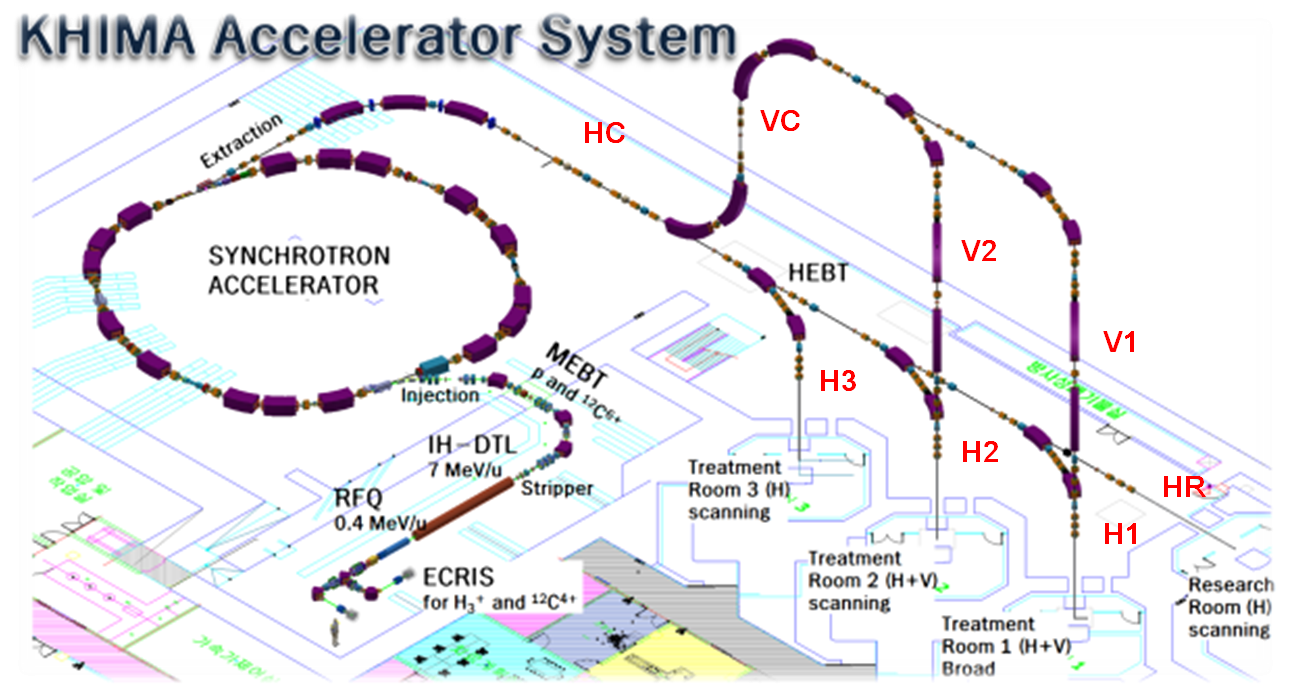
\includegraphics[width=8.0cm]{Fig01.png}
    \caption{(Color online) Schematic layout of the KHIMA accelerator system.}
    \label{fig0}
  \end{center}
\end{figure}
%---------------------------------------------------------------------------------------%
The electron cyclotron resounce ion source (ECRIS) generates ions with charge-to-mass ratio q/m = 1/3, in particular $H^{+}_{3}$ or $^{12}C^{4+}$, 
with energies up to 8.0 keV/$u$. 
These two ions are accelerated to 7 MeV/$u$ via the radio frequency quadrupole (RFQ) linac and the interdigital H-mode drift tube linac (IH-DTL). 
At the beginning of the medium energy beam transport (MEBT), each accelerated ion is fully ionized to either protons or a $^{12}C^{6+}$ 
and transported to the entrance of synchrotron to maintain a contant rate. 
Each ion is injected into a synchrotron having a multi-turn injection mechanism and is accelerated by the switching frequency on a radio frequency (RF) system. 
The accelerated ion beam is extracted to the high energy beam transport (HEBT) line using the slow resonance extraction method\cite{Extract,HJYim,Chawon}.
The beam extracted from the synchrotron is transported to each treatment room via a dedicated HEBT line as described in Sec.~\ref{sec:Lat}.
In Sec.~\ref{sec:TRACK}, two different beam tracking algorithms are introduced to realize beam dynamics in the HEBT line.
Finally the results and conclusions are given in Sec.~\ref{sec:Con}.
%---------------------------------------------------------------------------------------%
\section{Lattice Design}
\label{sec:Lat}
%---------------------------------------------------------------------------------------%
Beams extracted from the synchrotron must be safely transported to the isocenter in their own treatment rooms or research room.
To satisfy this requirement, the lattice design was conducted by two different beam optics codes, WinAgile\cite{Agile0,Agile1} and MAD-X\cite{Schmidt}.
Meanwhile, the distorted trajectory for several reasons was corrected by the beam optics tool\cite{Chawon}.
The common module of the horizontal common (HC) line is interleaved to control the beam size at the isocenter.
This module has important advantages for commissioning and operation. 
The vertical beam size of transverse beam plane at the isocenter is controlled by the vertical $\beta$ function, $\beta_{y}$.  
The module can be adjusted to provide a variable value between $2 < \beta_{y} < 27$ m with $\alpha_{y} = ~0$ at the isocenter. 
As a variable component, the module includes six successive quadrupole magnets in a common line.
The horizontal beam size of transversal beam plane was limited by changing the phase advance as described in ref.\cite{Chawon}. 
As the shortest of the horizontal lines (H3, H2 and H1), 
Fig.~\ref{fig1} shows the transverse envelope distribution by the horizontal H3 line to the isocenter of the third treatment room. 
The full width at half maximum (FWHM; $\Gamma$) at the isocenter can be varied with respect to the beam energy according to treatment conditions.
Thus, the lattice design reflects these conditions by arranging the corresponding lattice components which are bending, focusing and correcting magnets.
%---------------------------------------------------------------------------------------%
\begin{figure}[h]
  \begin{center}
    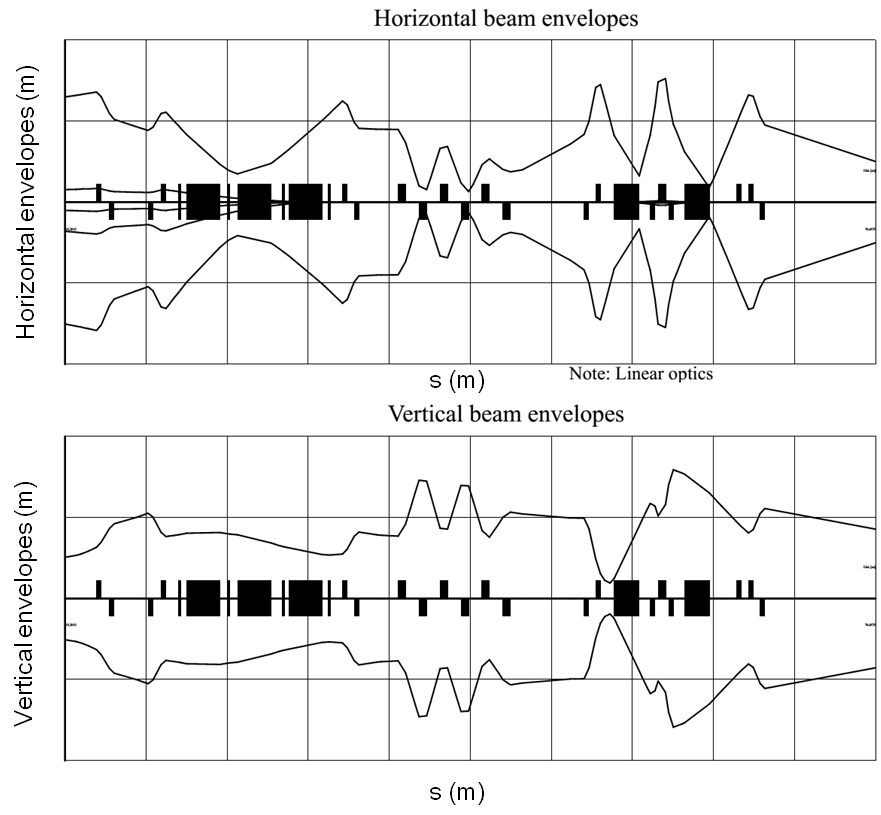
\includegraphics[width=7.5cm]{Fig02.png}  
    \caption{Beam envelope distribution of the third horizontal~(H3) line.
      There are restrictions when $\Gamma_{y} = 9$~mm with an isocenter using a carbon beam with E = 110 MeV/u.}
    \label{fig1}
  \end{center}
\end{figure}
%---------------------------------------------------------------------------------------%

%---------------------------------------------------------------------------------------%
\section{Beam tracking simulation}
\label{sec:TRACK}
%---------------------------------------------------------------------------------------%
A beam transport system such as the HEBT line is completed using a detailed beam dynamics code.
Due to many advantages, the ray tracing code TRACK\cite{TRACK} was adopted to describe the beam dynamics of the HEBT line.
In the beam tracking simulation by the TRACK code, two different methods are used firstly by the encoding algorithm embedded in the program
and secondly by the algorithm applying for the realistic field map in the electromagnets.
%%%%


\subsection{Encoded in TRACK Code}
In the hard-edge model of electromagnet, the fringe field falloff of the dipole and multipole magnet elements is not included.
On the other hand, the TRACK code implements the encoded 6 parameter Enge function\cite{Enge} and describes the parasitic fringe field component.  
The Enge function is described as\cite{EngeTrack}:
%\begin{equation}\label{eq:Enge}
\[
F(z) = \frac{1}{1+{\rm exp}(a_{0}+a_{1}(z/D)^{1}+...+a_{5}(z/D)^{5})} 
%\end{equation}
\]
where $z$ is the distance along the line perpendicular to the effective bounday line and $D$ is the full air-gap of element.
Fig.~\ref{fig2} shows the beam envelope distribution for the reference trajectory in both horizontal and vertical planes.
As shown in the distribution diagram on the lower right side of Fig.~\ref{fig3}, FWHM $\Gamma_{y} = 2.355 \times \sigma_{y} = 6.7$~mm was obtained
and the result by the matrix based optical code WinAgile was 9~mm.
Therefore, the difference between the two methods is large and needs to be considered for additional correction.
%---------------------------------------------------------------------------------------%
\begin{figure}[h]
  \begin{center}
    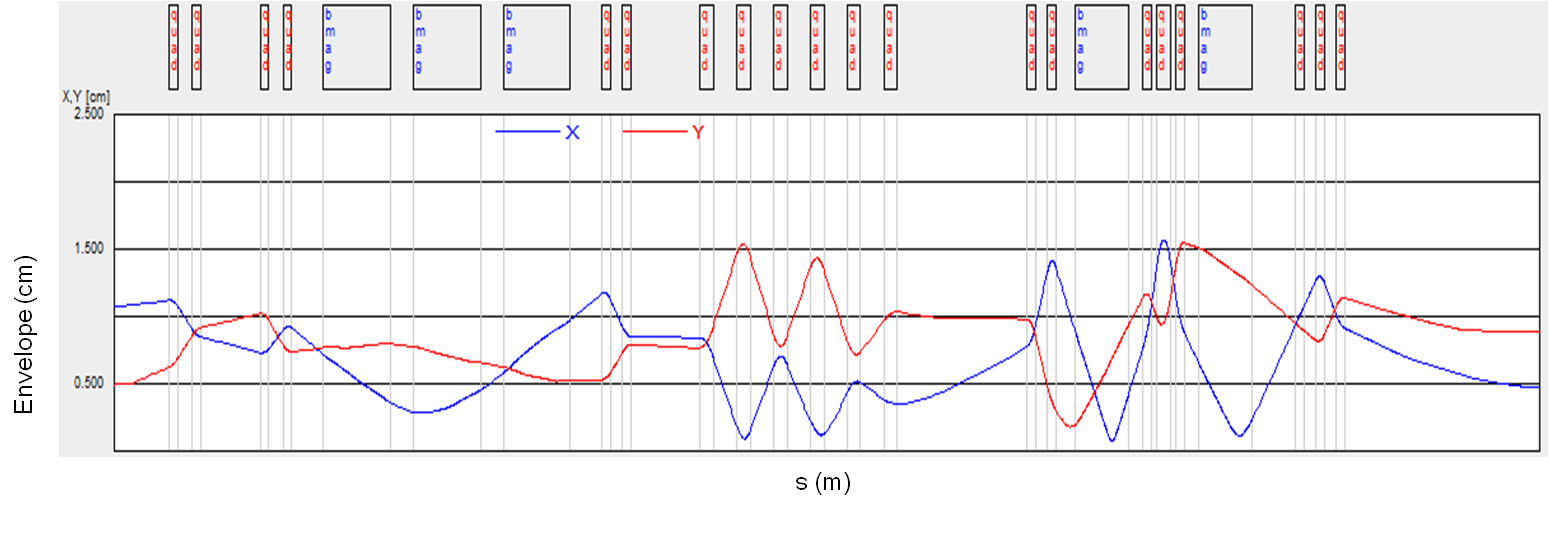
\includegraphics[width=8.5cm]{Fig03.png}      
    \caption{(Color online) Beam envelope distributions for the 3rd Horizontal (H3) line by using the encoded fringe field fall-off with TRACK, 
      where $\Gamma_{y} = 9$~mm with E = 110 MeV/u carbon beam at the iso-center is estimated by optics code.}
    \label{fig2}
  \end{center}
\end{figure}
%---------------------------------------------------------------------------------------%

%---------------------------------------------------------------------------------------%
\begin{figure}[h]
  \begin{center}
    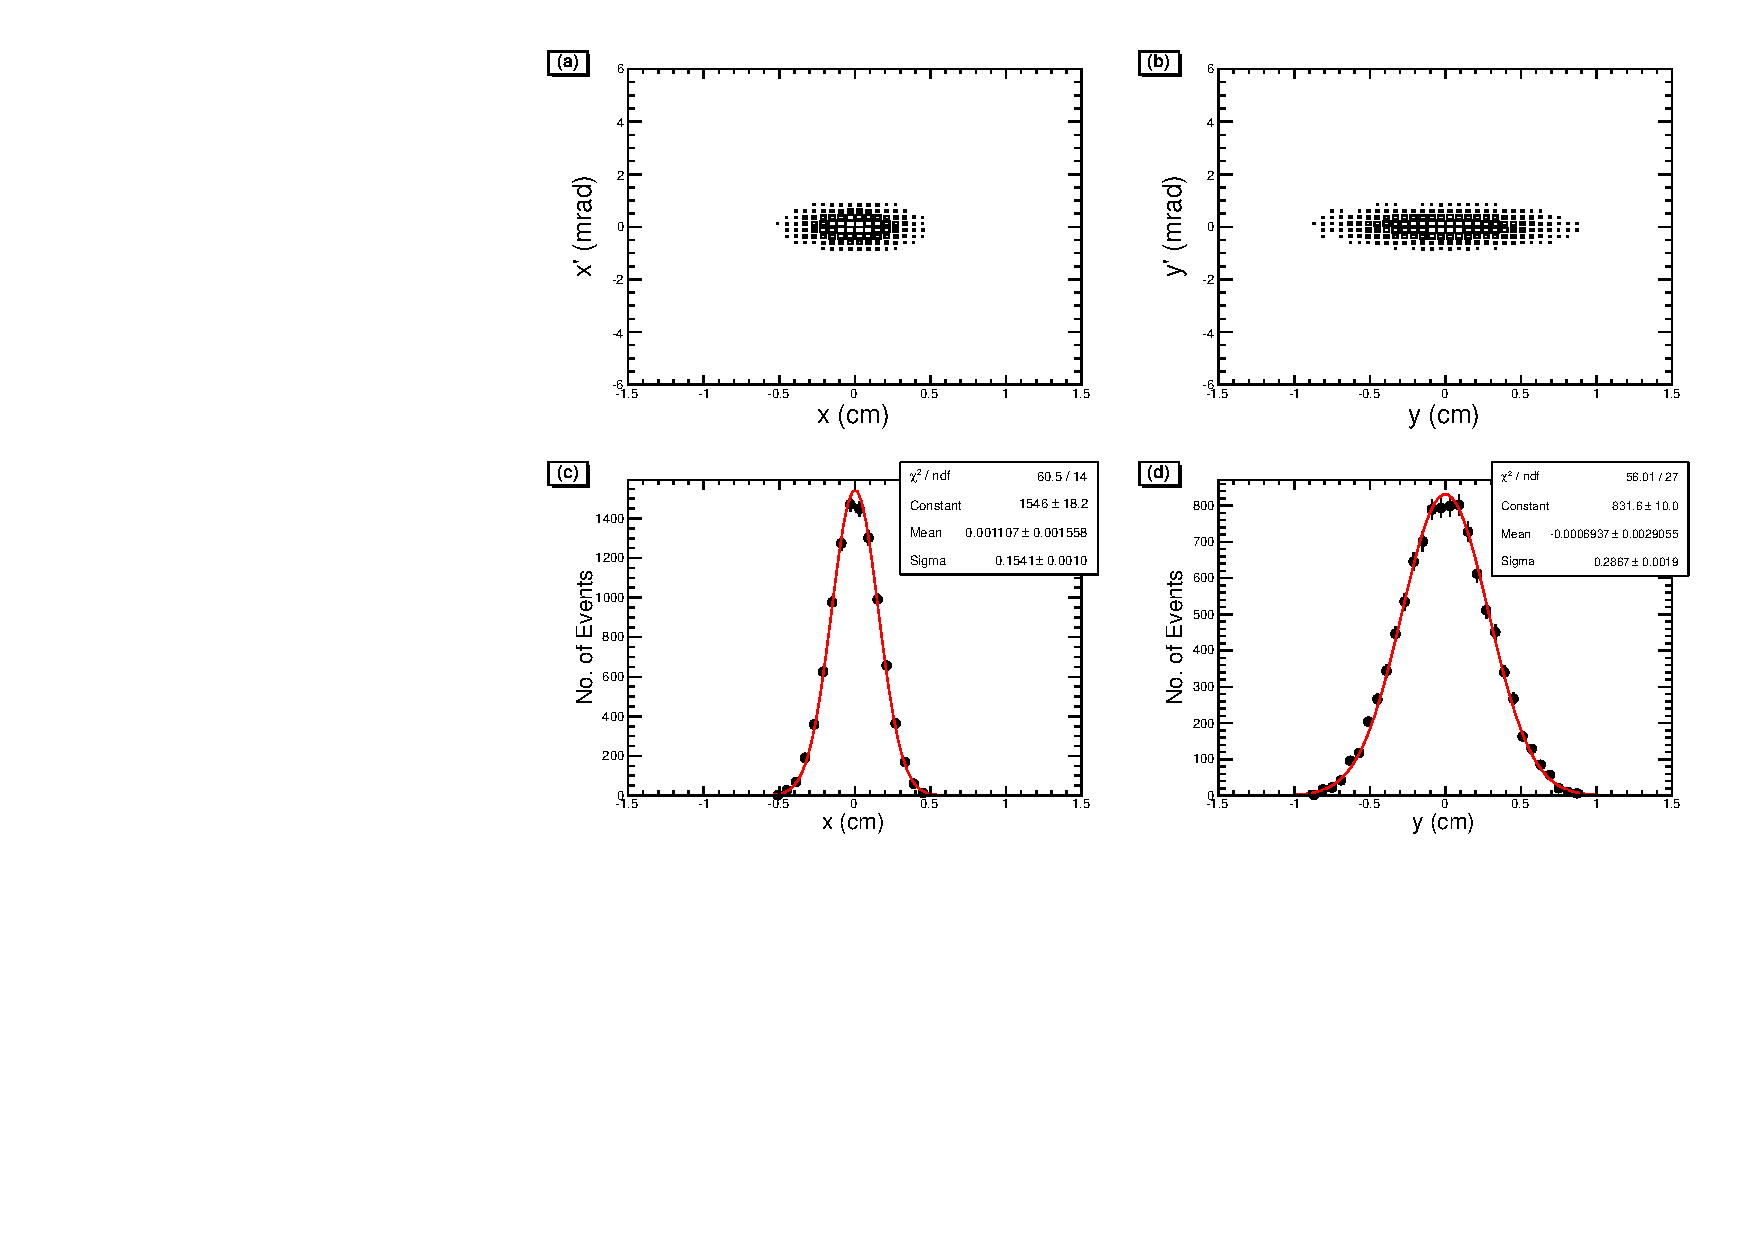
\includegraphics[width=8.5cm]{Fig04.pdf}
    \caption{(Color online) (a) - (b) Particle beam distribution at the isocenter in phase space. (c) - (d) Particle distribution projected on each x, y plane.}
    \label{fig3}
  \end{center}
\end{figure}
%---------------------------------------------------------------------------------------%

\subsection{Three Dimensional Field Map}
%---------------------------------------------------------------------------------------%
\begin{figure*}[t]
  \begin{center}
    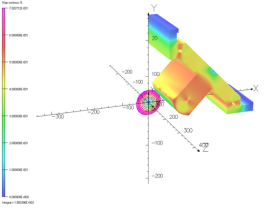
\includegraphics[width=6cm]{Fig04-1.png}
    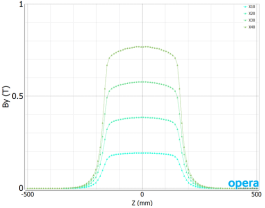
\includegraphics[width=6cm]{Fig04-2.png}
    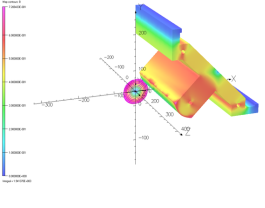
\includegraphics[width=6cm]{Fig04-3.png}
    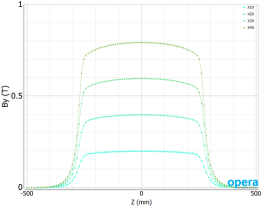
\includegraphics[width=6cm]{Fig04-4.png}
    \caption{(Color online) Schematic design output and field distribution
      over extreme points for short and long distance quadrupole.}
    \label{fig3-1}
  \end{center}
\end{figure*}
%---------------------------------------------------------------------------------------%
Design specifications of dipole and quadrupole determined by beam optics code are realized with Opera3D code.
Fig.~\ref{fig3-1} shows the schematic design and magnetic field distribution of two different quadrupole magnets. Here, the reason for using two different
focusing magnets is to respect the wide range magnetic strength of each quadrupole.
%Fig.~\ref{fig4} shows the distribution of field maps for three different bending angles 22.5 degrees, 30 degrees and 45 degrees used in the HEBT line.
Fig.~\ref{fig4} shows the distribution of field maps for three different bending angles 22.5$^{\circ}$, 30$^{\circ}$ and 45$^{\circ}$ used in the HEBT line.
%---------------------------------------------------------------------------------------%
\begin{figure}
  \begin{center}
    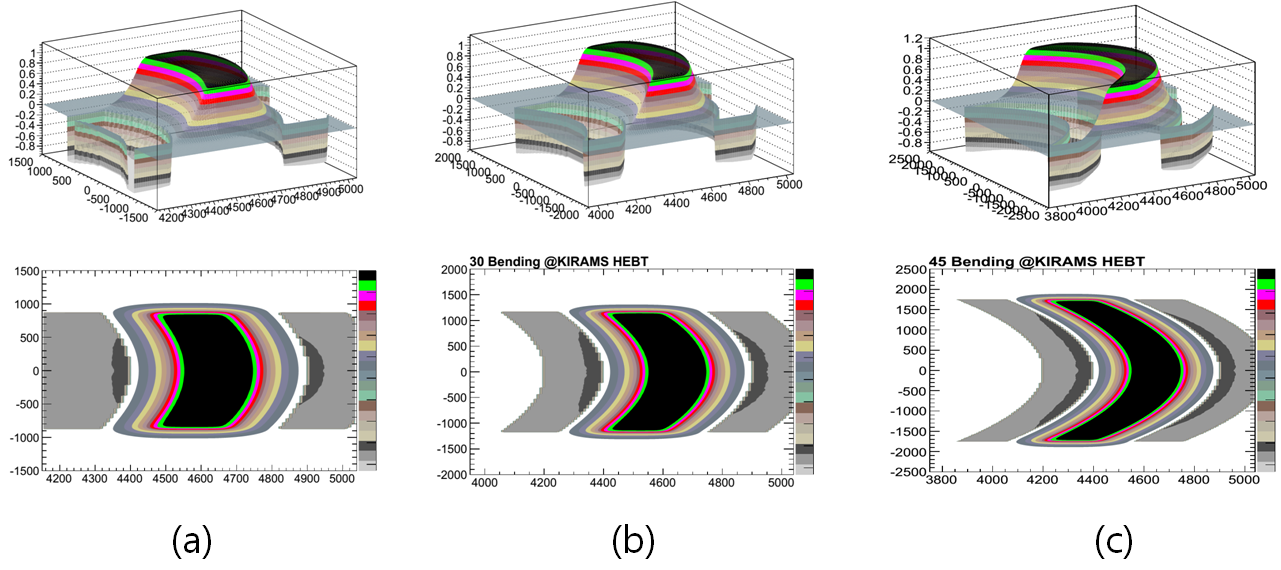
\includegraphics[width=8.0cm, height=4cm]{Fig05.png}
    \caption{(Color online) 3-D field map distribution of (a) 22.5$^{\circ}$, (b) 30$^{\circ}$ and (c) 45$^{\circ}$ bending magnet of Opera3D.}
    \label{fig4}
  \end{center}
\end{figure}
%---------------------------------------------------------------------------------------%
The field map database of multipole magnets from Opera3D code was converted into ASCII text input file of TRACK code.
In the TRACK code, two functions, three-dimensional bending and focusing magnet, are provided to read an ASCII text file.
The particle beam is transferred via the rewritten TRACK code applied by the field map implementation.
Fig.~\ref{fig5} shows the distribution of the particle beam envelope by applying the three-dimensional magnetic field map realized by the multipole magnet to the TRACK code.
Even if the realized field map is applied, the isocenter's FWHM value still does not match the field map expected by the beam optics code.
Fig.~\ref{fig6} shows the discrepancy of the FWHM distribution between the reconstruction value according to the TRACK code
and the estimate by the optics code for various carbon energies from 110 MeV/u to 430 MeV/u.   
The main reason for disagreement was derived from the fringe field effect in each quadrupole magnet.
%---------------------------------------------------------------------------------------%
\begin{figure}[h]
  \begin{center}
    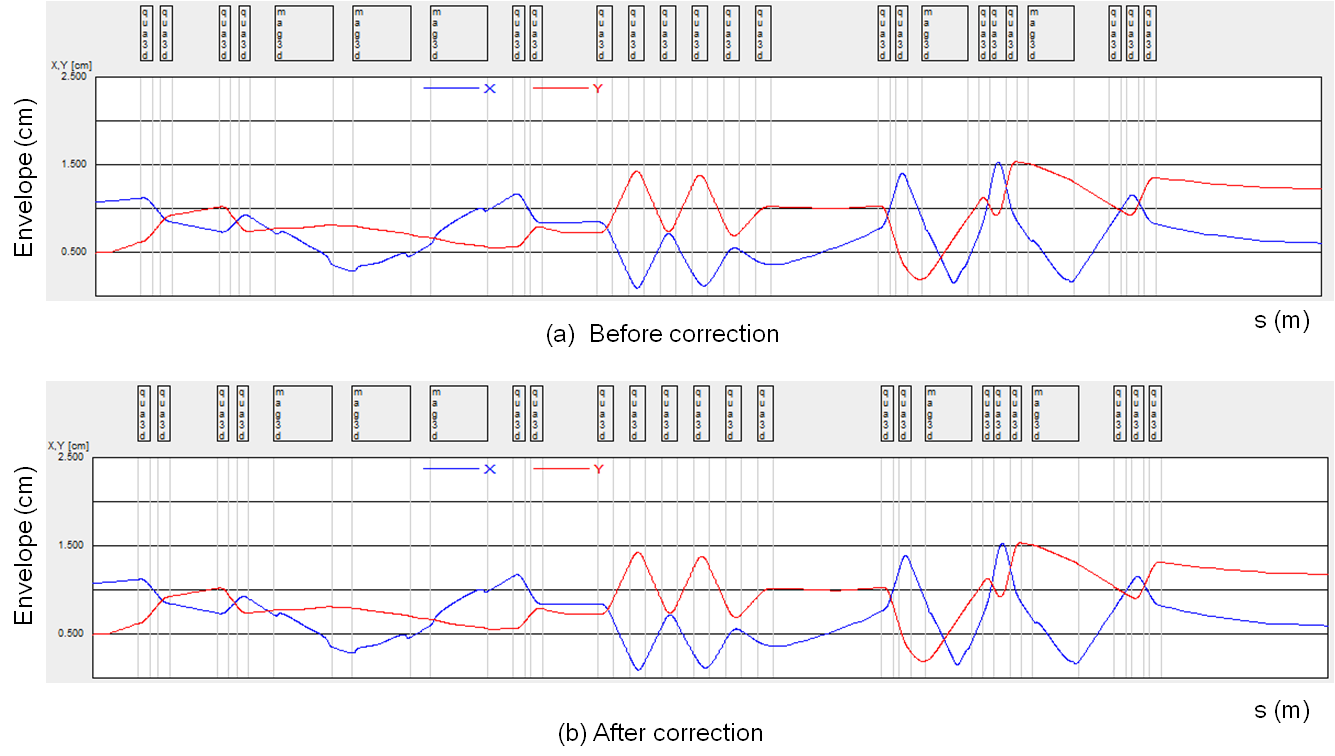
\includegraphics[width=8.0cm]{Fig06.png}    
    \caption{(Color online) Beam envelope of the 3rd Horizontal (H3) line using the 3-D field map with Opera3D code before and after correction.
      Here we set $\Gamma_{y} = 9$~mm using a carbon beam with E = 110 MeV/u at the isocenter.}
    \label{fig5}
  \end{center}
\end{figure}
%---------------------------------------------------------------------------------------%
%---------------------------------------------------------------------------------------%
\begin{figure}[h]
  \begin{center}
    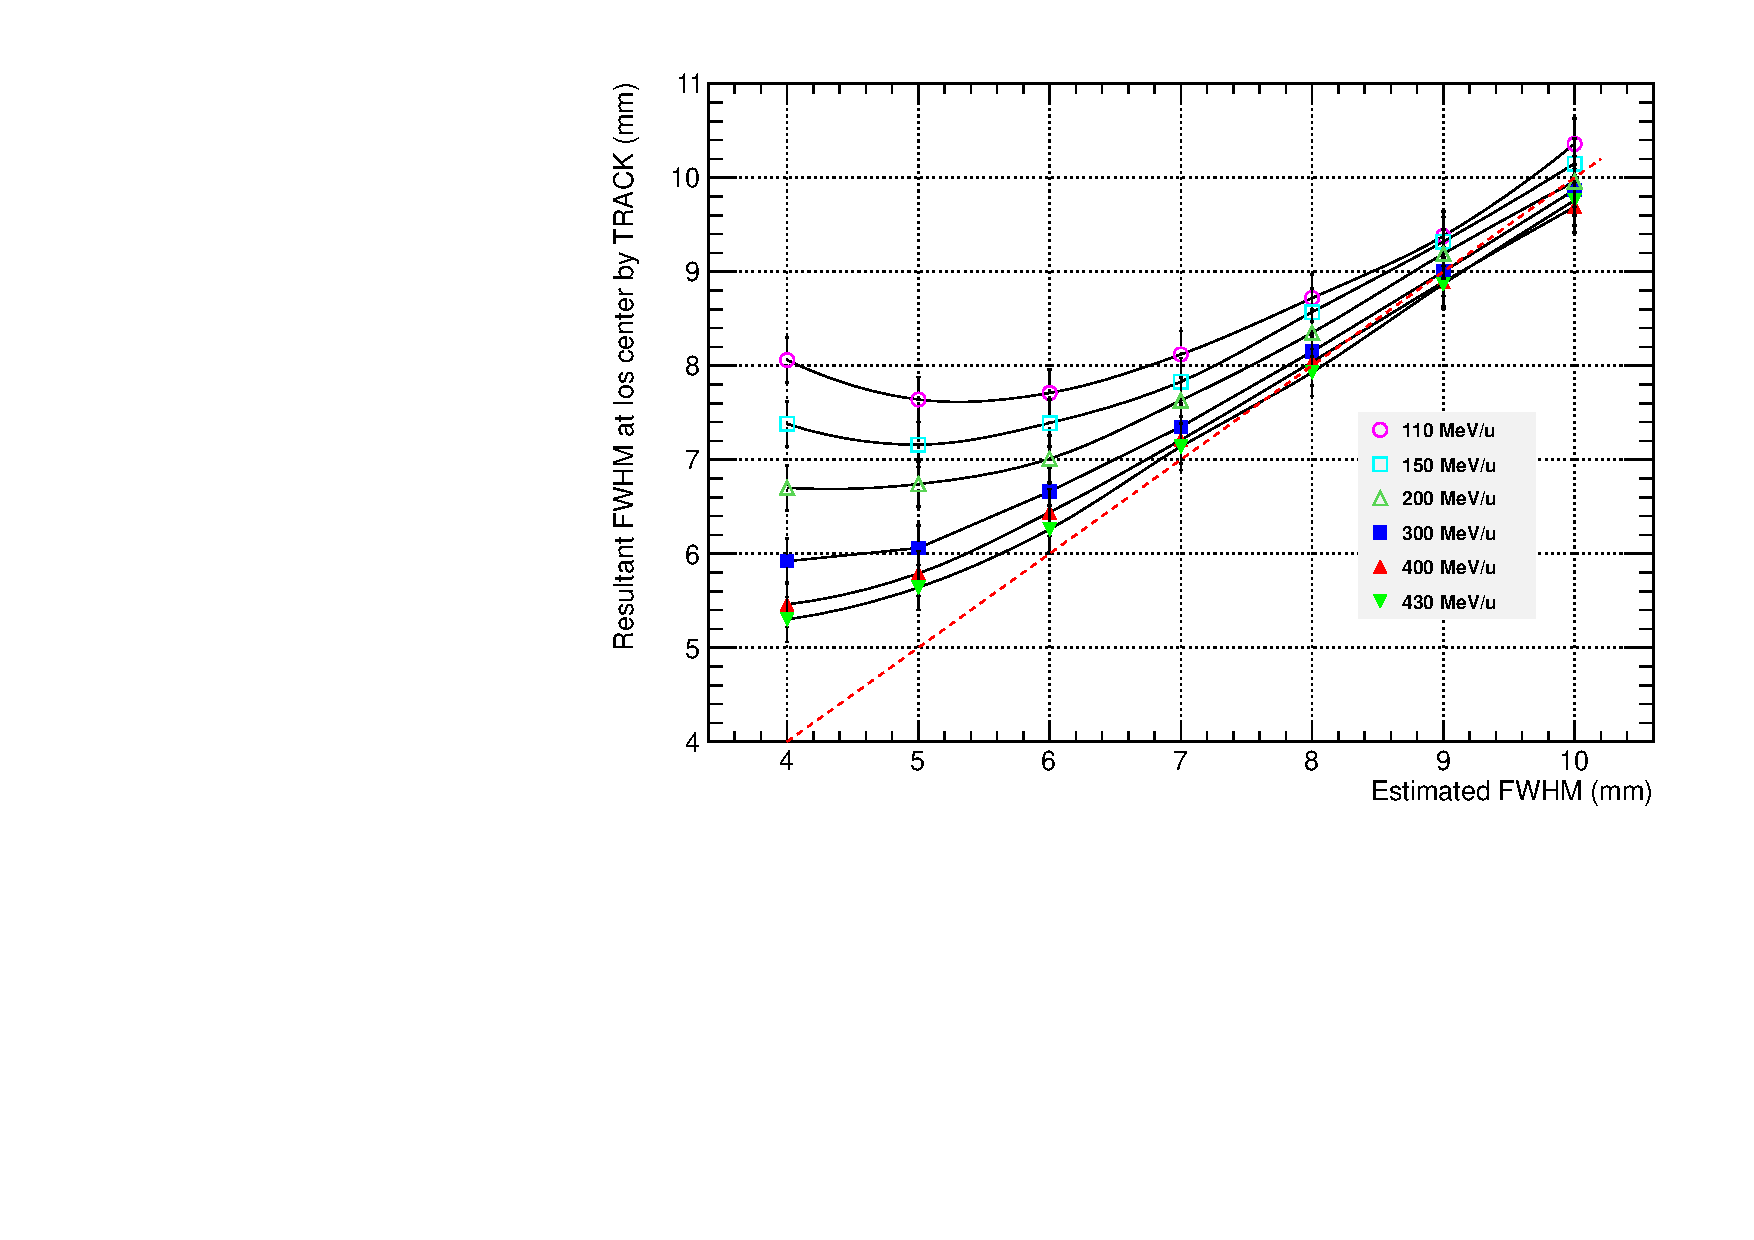
\includegraphics[width=8.5cm]{Fig06-1.pdf}    
    \caption{(Color online) FWHM distribution for the estimated one by the optical code at the isocenter
      for several energies of the carbon beam.}
    \label{fig6}
  \end{center}
\end{figure}
%---------------------------------------------------------------------------------------%
%---------------------------------------------------------------------------------------%
\begin{figure}[h]
  \begin{center}
    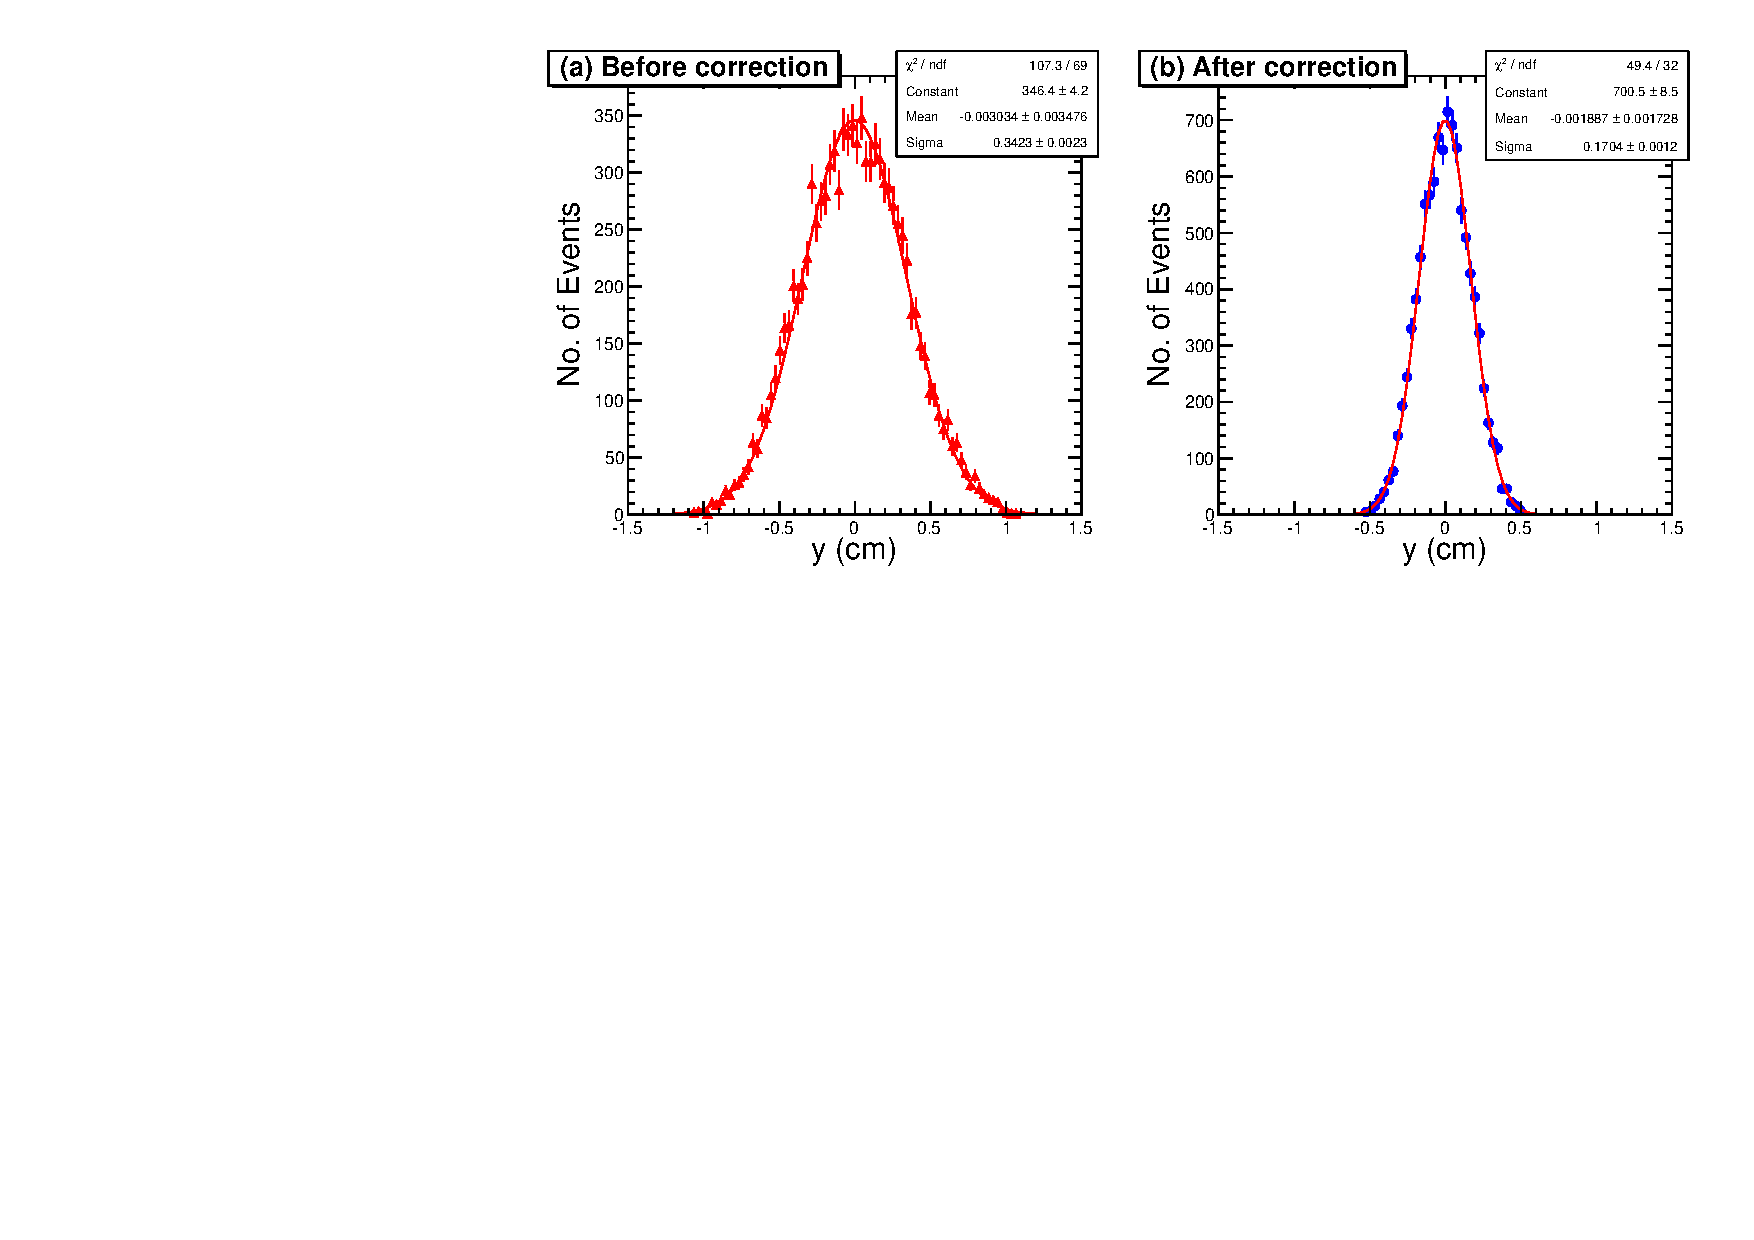
\includegraphics[width=8.5cm]{Fig08-1.pdf}
    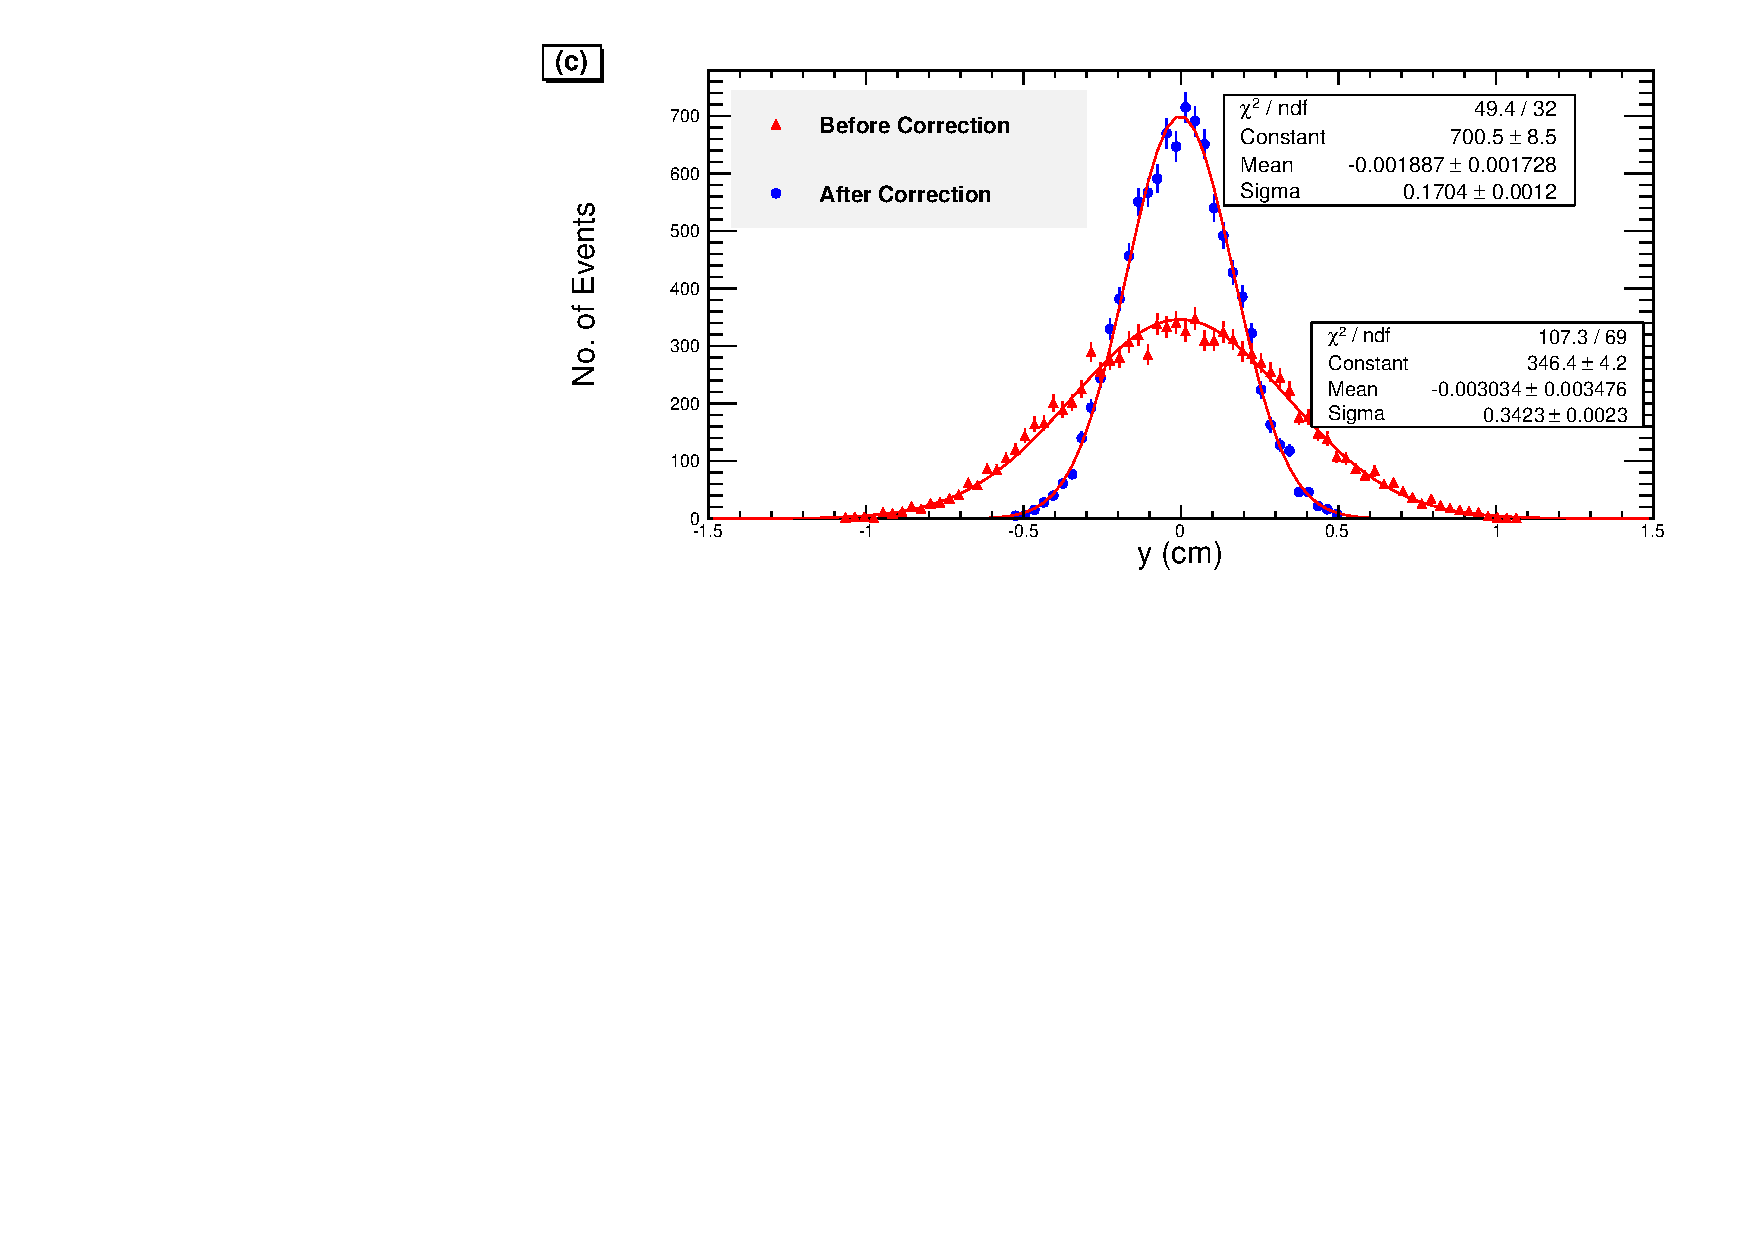
\includegraphics[width=8.5cm]{Fig08-2.pdf}        
    \caption{(Color online) Particle distribution projected on y plane before and after correction.
      Here we set $\Gamma_{y} = 4$~mm using a carbon beam with E = 110 MeV/u at the isocenter.}
    \label{fig7}
  \end{center}
\end{figure}
%---------------------------------------------------------------------------------------%
Various correction methods of the quadrupole magnets are considered to correct the mismatch,
but the field scaling factor multiplied to the quadrupole being used is most appropriate for the H3 line.
As an example, Fig.~\ref{fig7} shows the particle distribution projected on y plane before and after the correction.
%Here we set $\Gamma_{y} = 4$~mm (sigma, $\sigma_{y} = \Gamma_{y}/2.355 = 0.1699$ mm) using a carbon beam with E = 110 MeV/u at the isocenter.
%The fitted sigma ($\sigma_{y}$ = 0.1704 $\pm$ 0.0012 mm) value after correction is consistent with the value estimated by the optical code within statistical fluctuation.
Here we set $\Gamma_{y} = 4$~mm (sigma, $\sigma_{y} = \Gamma_{y}/2.355 = 0.170$ mm) using a carbon beam with E = 110 MeV/u at the isocenter.
The fitted sigma ($\sigma_{y}$ = 0.170 $\pm$ 0.001 mm) value after correction is consistent with the value estimated by the optical code within statistical fluctuation.

Fig.~\ref{fig8} shows the performance of particle beam width for extremely different beam energies before and after correction.
As shown in Fig.~\ref{fig8}, the correction factor, which is inversely proportional to the ratio of the figure, in the low carbon energy beam
must be greater than that of the high energy beam.
%---------------------------------------------------------------------------------------%
\begin{figure}[h]
  \begin{center}
    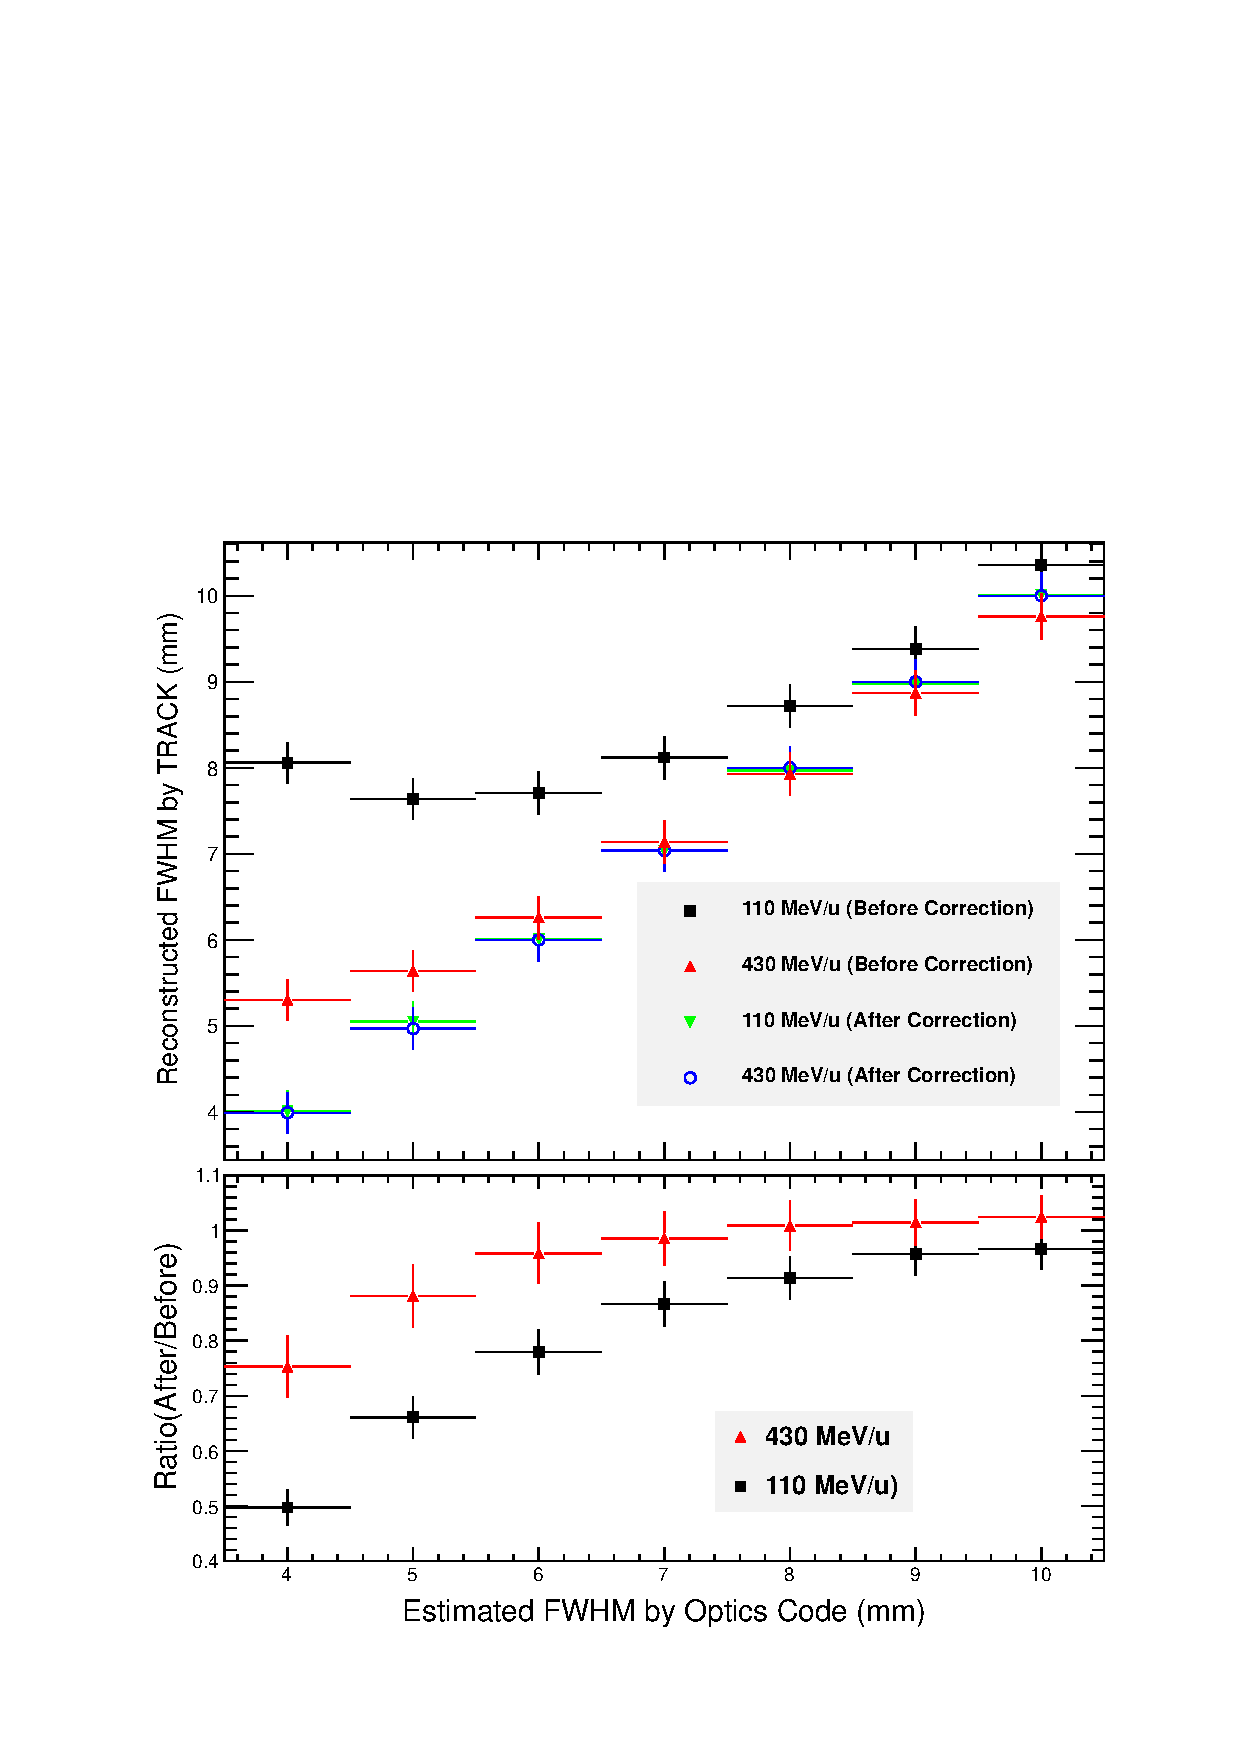
\includegraphics[width=8.1cm]{Fig07-1.pdf}
    \caption{(Color online) Reconstructed FWHM distribution estimated by optical code (WinAgile) at the isocenter before and after correction    
      of the minimum and maximum energy of the carbon beam.}
    \label{fig8}
  \end{center}
\end{figure}
%---------------------------------------------------------------------------------------%
In the treatment planning system (TPS), combinations of hundreds of thousands of beam are required,
including the number of ion species, different energies, beam size, intensity and extraction time.
Based on this analysis with TRACK code, tracking analysis is also successfully performed by other beam lines on the HEBT.
Thus, the transportation of the beam to the isocenter through each line works well with suitable and variable magnet components without beam loss.
%\newpage

\section{Conclusion}
\label{sec:Con}
The HEBT line is constructed based on a modular design that takes into account the strong asymmetry
between two lateral emittiances in the lateral beam direction and depends on the trapezoidal distribution of the beam in the horizontal phase space.
The KHIMA HEBT line was originally designed using the WinAgile/Mad-X code for the whole beam transport line to each treatment room.
Optical code based designs were modified with appropriate correction methods for various treatment conditions. 
In order to confirm the design based on the optical code and minimize the beam loss in the transport line, tracking analysis using the TRACK code was carried out.
TPS requires an enormous amount of beam combinations and needs to be corrected appropriately.
In the beam commissioning process, various calibrations and corrections that affect beam performance are performed.
Therefore, tracking analysis using the realized three-dimensional electromagnetic field map is very useful
for performing correction of each electromagnetic magnet component in the beam commissioning process.
Designed beam lines are expected to be built on the basis of optical codes and tracking codes in the near future.
\section{acknowledgment}
This work was supported by the National Research and Development Program through the Korea Institute of Radiological and Medical Sciences
%funded by the Ministry of Science, ICT \& Future Planning (NRF-2015M2C3A1001637).
funded by the Ministry of Science, ICT \& Future Planning (NRF-2014M2C3A1029534).

%---------------------------------------------------------------------------------------%
%\newpage
%---------------------------------------------------------------------------------------%
\begin{references}
\bibitem{HJYim} Heejoong Yim {\it et al.}, J. Korean Phys. Soc. {\bf 67}, 1364(2015).
\bibitem{Chawon} Chawon Park, Heejoong Yim, Garam Hahn and Dong Hyun An {\it et al.}, J. Korean Phys. Soc. {\bf 69}, 933(2016).   
\bibitem{Extract} M. Benedikt {\it et al.}, Nucl. Instrum. Methods Phys. Res. A {\bf 430}, 523 (1999). 
%\bibitem{MBenedikt01} M. Benedikt, ``Optics design of the extraction lines for the MedAustron hadron therapy centre'', 
%  Nucl. Instrum. Methods A 430 {\bf 512-522} (1999).
\bibitem{Agile0} P. Bryant, {\it AGILE, a tool for interactive lattice design: Proceedings, 7th European Conference, EPAC2000}, p.1357-1359.
\bibitem{Agile1} P. J. Bryant, {\it AGILE program for synchrotron lattice design}, http://nicewwww.cern.ch/bryant.  
\bibitem{Schmidt} F. Schmidt and H. Grote, ``MAD X an update from MAD8'', Proc. Part. Acc. Conference, Portland, U.S.A, 12.-16.5, {\bf 3497} (2003).  
\bibitem{TRACK} P. N. Ostroumov and K. W. Shepard, Phys. Rev. ST. Accel. Beams 11, 030101 (2001).
\bibitem{Enge} H. A. Enge, Rev. of Sci. Instr. {\bf 35}, 278 (1964).  
\bibitem{EngeTrack} P. N. Ostroumov, V. N. Aseev, and B. Mustapha, {\it TRACK - a Code for Beam Dynamics Simulation in Accelerators and Transport Lines with 3D Electric and Magnetic Fields}, Technical Note (ver. 3.7), Mar. 2007, pp. 6.  
\end{references}
%---------------------------------------------------------------------------------------%
\end{document}
